\documentclass[12pt, oneside]{article}

\usepackage[letterpaper, scale=0.89, centering]{geometry}
\usepackage{fancyhdr}
\setlength{\parindent}{0em}
\setlength{\parskip}{1em}

\usepackage{tikz}
\usetikzlibrary{automata,positioning,arrows}

\pagestyle{fancy}
\fancyhf{}
\renewcommand{\headrulewidth}{0pt}
\rfoot{\href{https://creativecommons.org/licenses/by-nc-sa/2.0/}{CC BY-NC-SA 2.0} Version \today~(\thepage)}

\usepackage{amssymb,amsmath,pifont,amsfonts,comment,enumerate,enumitem}
\usepackage{currfile,xstring,hyperref,tabularx,graphicx,wasysym}
\usepackage[labelformat=empty]{caption}
\usepackage{xcolor}
\usepackage{multicol,multirow,array,listings,tabularx,lastpage,textcomp,booktabs}

\lstnewenvironment{algorithm}[1][] {   
    \lstset{ mathescape=true,
        frame=tB,
        numbers=left, 
        numberstyle=\tiny,
        basicstyle=\rmfamily\scriptsize, 
        keywordstyle=\color{black}\bfseries,
        keywords={,procedure, div, for, to, input, output, return, datatype, function, in, if, else, foreach, while, begin, end, }
        numbers=left,
        xleftmargin=.04\textwidth,
        #1
    }
}
{}

\newcommand\abs[1]{\lvert~#1~\rvert}
\newcommand{\st}{\mid}

\newcommand{\cmark}{\ding{51}}
\newcommand{\xmark}{\ding{55}}
 
\begin{document}
\begin{flushright}
    \StrBefore{\currfilename}{.}
\end{flushright} \section*{Day15}


We are ready to introduce a formal model that will capture a notion of general purpose computation.
\begin{itemize}
\item {\it Similar to DFA, NFA, PDA}: input will be an arbitrary string over a fixed alphabet.
\item {\it Different from NFA, PDA}: machine is deterministic.
\item {\it Different from DFA, NFA, PDA}: read-write head can move both to the left and to the right,
and can extend to the right past the original input.
\item {\it Similar to DFA, NFA, PDA}: transition function drives computation one step at a time 
by moving within a finite set of states, always starting at designated start state.
\item {\it Different from DFA, NFA, PDA}: the special states for rejecting and accepting take effect immediately.
\end{itemize}

\vspace{-10pt}

(See more details: Sipser p. 166)

\vfill

Formally: a  Turing machine is $M= (Q, \Sigma, \Gamma, \delta, q_0, q_{accept}, q_{reject})$ 
where $\delta$ is the {\bf transition function} 
\[
  \delta: Q\times \Gamma \to Q \times \Gamma \times \{L, R\}
\]
The {\bf computation} of $M$ on a string $w$ over $\Sigma$  is:

\vspace{-10pt}

\begin{itemize}
\setlength{\itemsep}{0pt}
\item Read/write head starts at leftmost position on tape. 
\item Input string is written on $|w|$-many leftmost cells of tape, 
rest of  the tape cells have  the blank symbol. {\bf Tape alphabet} 
is $\Gamma$ with $\textvisiblespace\in \Gamma$ and $\Sigma \subseteq \Gamma$.
The blank symbol $\textvisiblespace \notin \Sigma$.
\item Given current state of machine and current symbol being read at the tape head, 
the machine transitions to next state, writes a symbol to the current position  of the 
tape  head (overwriting existing symbol), and moves the tape head L or R (if possible). 
\item Computation ends {\bf if and when} machine enters either the accept or the reject state.
This is called {\bf halting}.
Note: $q_{accept} \neq q_{reject}$.
\end{itemize}

The {\bf language recognized by the  Turing machine} $M$,  is  $L(M) = \{ w \in \Sigma^* \mid w \textrm{ is accepted by } M\}$,
which is defined as
\[
  \{ w \in \Sigma^* \mid \textrm{computation of $M$ on $w$ halts after entering the accept state}\}
\]




\newpage
\begin{multicols}{2}
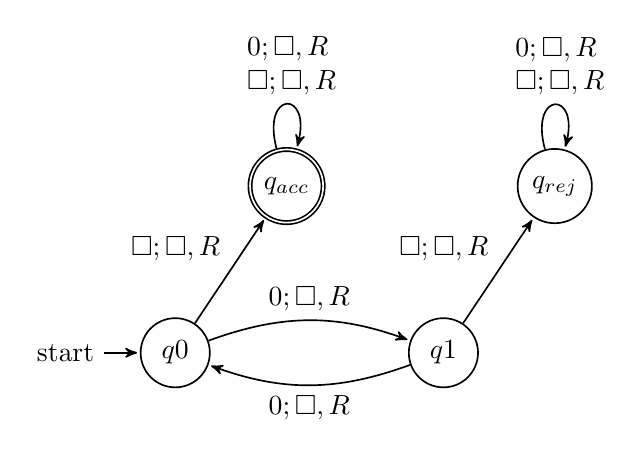
\begin{tikzpicture}[->,>=stealth',shorten >=1pt, auto, node distance=2cm, semithick]
  \tikzstyle{every state}=[text=black, fill=none]
  
  \node[initial,state] (q0)          {$q0$};
  \node[state]         (q1) [right of=q0, xshift=40pt] {$q1$};
  \node[state,accepting]         (qacc) [above right of=q0, yshift=20pt] {$q_{acc}$};
  \node[state]         (qrej) [above right of=q1,yshift=20pt] {$q_{rej}$};
  
  \path (q0) edge [bend left=0] node {$\square; \square, R$} (qacc)
      (q0) edge  [bend left=20] node {$0; \square, R$} (q1)
      (q1) edge [bend left=20] node {$0; \square, R$} (q0)
      (q1) edge [bend left=0] node {$\square; \square, R$} (qrej)
      (qacc) edge  [loop above] node {\parbox{1cm}{$0; \square, R$\newline $\square; \square, R$}} (qacc)
      (qrej) edge  [loop above] node {\parbox{1cm}{$0; \square, R$\newline $\square; \square, R$}}  (qrej)
  ;
\end{tikzpicture}
\columnbreak

Formal definition:

\vspace{10pt}

Sample computation: 

\begin{tabular}{|c|c|c|c|c|c|c|}
\hline
\multicolumn{1}{|c}{$q0\downarrow$} &  \multicolumn{6}{c|}{\phantom{A}}\\
\hline
$0$ & $0$  & $0$ & $\textvisiblespace $& $\textvisiblespace $& $\textvisiblespace $&  $\textvisiblespace $\\
\hline
\multicolumn{7}{|c|}{\phantom{A}}\\
\hline
\phantom{AA} & \phantom{AA}& \phantom{AA}& \phantom{AA}& \phantom{AA}& \phantom{AA}& \phantom{AA} \\
\hline
\multicolumn{7}{|c|}{\phantom{A}}\\
\hline
\phantom{AA} & \phantom{AA}& \phantom{AA}& \phantom{AA}& \phantom{AA}& \phantom{AA}& \phantom{AA} \\
\hline
\multicolumn{7}{|c|}{\phantom{A}}\\
\hline
\phantom{AA} & \phantom{AA}& \phantom{AA}& \phantom{AA}& \phantom{AA}& \phantom{AA}& \phantom{AA} \\
\hline
\multicolumn{7}{|c|}{\phantom{A}}\\
\hline
\phantom{AA} & \phantom{AA}& \phantom{AA}& \phantom{AA}& \phantom{AA}& \phantom{AA}& \phantom{AA} \\
\hline
\end{tabular}
\end{multicols}
\vfill

The language recognized by this machine is \ldots

\vfill
 

{\bf Describing  Turing machines} (Sipser p. 185) To define a Turing machine, we could give a 
\begin{itemize}
\item {\bf Formal definition}: the $7$-tuple of parameters including set of states, 
input alphabet, tape alphabet, transition function, start state, accept state, and reject state; or,
\item {\bf Implementation-level definition}: English prose that describes the Turing machine head 
movements relative to contents of tape, and conditions for accepting / rejecting based on those contents.
\item {\bf High-level description}: description of algorithm (precise sequence of instructions), 
without implementation details of machine. As part of this description, can ``call" and run 
another TM as a subroutine.
\end{itemize}
  
\newpage
Fix $\Sigma = \{0,1\}$, $\Gamma = \{ 0, 1, \textvisiblespace\}$ for the Turing machines with  the following state diagrams:
  
\begin{center}
  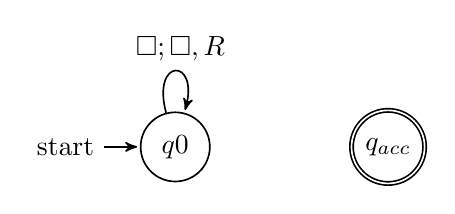
\begin{tikzpicture}[->,>=stealth',shorten >=1pt, auto, node distance=2cm, semithick]
    \tikzstyle{every state}=[text=black, fill=none]
    
    \node[initial,state] (q0)          {$q0$};
    \node[state,accepting]         (qacc) [right of=q0, xshift=20pt] {$q_{acc}$};
    
    \path (q0) edge  [loop above] node {\parbox{1cm}{$\square; \square, R$}} (q0)
    ;
  \end{tikzpicture}
\end{center}

Example of string accepted: \\
Example of string rejected: \\


Implementation-level description

\vfill

High-level description

\vfill

\begin{center}
  \begin{tikzpicture}[->,>=stealth',shorten >=1pt, auto, node distance=2cm, semithick]
    \tikzstyle{every state}=[text=black, fill=none]
    
    \node[initial,state] (qrej)          {$q_{rej}$};
    \node[state,accepting]         (qacc) [right of=q0, xshift=20pt] {$q_{acc}$};
  \end{tikzpicture}
\end{center}

Example of string accepted: \\
Example of string rejected: \\


Implementation-level description

\vfill

High-level description

\vfill

\newpage
\begin{center}
  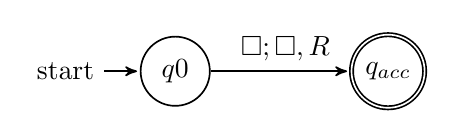
\begin{tikzpicture}[->,>=stealth',shorten >=1pt, auto, node distance=2cm, semithick]
    \tikzstyle{every state}=[text=black, fill=none]
    
    \node[initial,state] (q0)          {$q0$};
    \node[state,accepting]         (qacc) [right of=q0, xshift=20pt] {$q_{acc}$};
    
    \path (q0) edge  [bend left=0] node {\parbox{1cm}{$\square; \square, R$}} (qacc)
    ;
  \end{tikzpicture}
\end{center}

Example of string accepted: \\
Example of string rejected: \\


Implementation-level description

\vfill

High-level description

\vfill

\begin{center}
  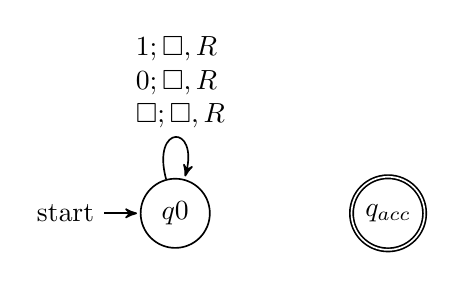
\begin{tikzpicture}[->,>=stealth',shorten >=1pt, auto, node distance=2cm, semithick]
    \tikzstyle{every state}=[text=black, fill=none]
    
    \node[initial,state] (q0)          {$q0$};
    \node[state,accepting]         (qacc) [right of=q0, xshift=20pt] {$q_{acc}$};
    
    \path (q0) edge  [loop above] node {\parbox{1cm}{$1; \square, R$\\$0; \square, R$\\$\square; \square, R$}} (q0)
    ;
  \end{tikzpicture}
\end{center}

Example of string accepted: \\
Example of string rejected: \\


Implementation-level description

\vfill

High-level description

\vfill

\newpage
 \vfill
\section*{Day16}



{\it Sipser Figure  3.10}

{\bf Conventions in state diagram of TM}: $b \to R$ label means $b \to b, R$ and
all arrows missing from diagram represent transitions with output $(q_{reject}, \textvisiblespace , R)$

\begin{multicols}{2}
\vspace{-20pt}
\begin{center}
\includegraphics[width=4in]{../../resources/machines/Lect13TM3.png}
\end{center}

Implementation level description of this machine:
\begin{quote}
Zig-zag across tape to corresponding positions on either side of $\#$ to check whether the 
characters in these positions agree. If they do not, or if there is no $\#$, reject. If they 
do, cross them off.

Once all symbols to the left of the $\#$ are crossed off, check for any un-crossed-off symbols 
to the right of $\#$; if there are any, reject; if there aren't, accept.
\end{quote}

The language recognized by this machine is
\[
  \{ w \# w \mid w \in \{0,1\}^* \}
\]

\columnbreak

Computation on  input  string  $01\#01$

\begin{tabular}{|c|c|c|c|c|c|c|}
\hline
\multicolumn{1}{|c}{$q_1 \downarrow$} &  \multicolumn{6}{c|}{\phantom{A}}\\
\hline
$0$ & $1$  & $\#$  & $0$ & $1$ & $\textvisiblespace $& $\textvisiblespace $\\
\hline
  \multicolumn{7}{|c|}{\phantom{A}}\\
  \hline
  \phantom{AA} & \phantom{AA}& \phantom{AA}& \phantom{AA}& \phantom{AA}& \phantom{AA}& \phantom{AA} \\
  \hline
  \multicolumn{7}{|c|}{\phantom{A}}\\
  \hline
  \phantom{AA} & \phantom{AA}& \phantom{AA}& \phantom{AA}& \phantom{AA}& \phantom{AA}& \phantom{AA} \\
  \hline
  \multicolumn{7}{|c|}{\phantom{A}}\\
  \hline
  \phantom{AA} & \phantom{AA}& \phantom{AA}& \phantom{AA}& \phantom{AA}& \phantom{AA}& \phantom{AA} \\
  \hline
  \multicolumn{7}{|c|}{\phantom{A}}\\
  \hline
  \phantom{AA} & \phantom{AA}& \phantom{AA}& \phantom{AA}& \phantom{AA}& \phantom{AA}& \phantom{AA} \\
  \hline
  \multicolumn{7}{|c|}{\phantom{A}}\\
  \hline
  \phantom{AA} & \phantom{AA}& \phantom{AA}& \phantom{AA}& \phantom{AA}& \phantom{AA}& \phantom{AA} \\
  \hline
  \multicolumn{7}{|c|}{\phantom{A}}\\
  \hline
  \phantom{AA} & \phantom{AA}& \phantom{AA}& \phantom{AA}& \phantom{AA}& \phantom{AA}& \phantom{AA} \\
  \hline
  \multicolumn{7}{|c|}{\phantom{A}}\\
  \hline
  \phantom{AA} & \phantom{AA}& \phantom{AA}& \phantom{AA}& \phantom{AA}& \phantom{AA}& \phantom{AA} \\
  \hline
  \multicolumn{7}{|c|}{\phantom{A}}\\
  \hline
  \phantom{AA} & \phantom{AA}& \phantom{AA}& \phantom{AA}& \phantom{AA}& \phantom{AA}& \phantom{AA} \\
  \hline
  \multicolumn{7}{|c|}{\phantom{A}}\\
  \hline
  \phantom{AA} & \phantom{AA}& \phantom{AA}& \phantom{AA}& \phantom{AA}& \phantom{AA}& \phantom{AA} \\
  \hline
  \multicolumn{7}{|c|}{\phantom{A}}\\
  \hline
  \phantom{AA} & \phantom{AA}& \phantom{AA}& \phantom{AA}& \phantom{AA}& \phantom{AA}& \phantom{AA} \\
  \hline
  \multicolumn{7}{|c|}{\phantom{A}}\\
  \hline
  \phantom{AA} & \phantom{AA}& \phantom{AA}& \phantom{AA}& \phantom{AA}& \phantom{AA}& \phantom{AA} \\
  \hline
  \multicolumn{7}{|c|}{\phantom{A}}\\
  \hline
  \phantom{AA} & \phantom{AA}& \phantom{AA}& \phantom{AA}& \phantom{AA}& \phantom{AA}& \phantom{AA} \\
  \hline
  \multicolumn{7}{|c|}{\phantom{A}}\\
  \hline
  \phantom{AA} & \phantom{AA}& \phantom{AA}& \phantom{AA}& \phantom{AA}& \phantom{AA}& \phantom{AA} \\
  \hline
  \multicolumn{7}{|c|}{\phantom{A}}\\
  \hline
  \phantom{AA} & \phantom{AA}& \phantom{AA}& \phantom{AA}& \phantom{AA}& \phantom{AA}& \phantom{AA} \\
  \hline
  \multicolumn{7}{|c|}{\phantom{A}}\\
  \hline
  \phantom{AA} & \phantom{AA}& \phantom{AA}& \phantom{AA}& \phantom{AA}& \phantom{AA}& \phantom{AA} \\
  \hline
  \multicolumn{7}{|c|}{\phantom{A}}\\
  \hline
  \phantom{AA} & \phantom{AA}& \phantom{AA}& \phantom{AA}& \phantom{AA}& \phantom{AA}& \phantom{AA} \\
  \hline
  \multicolumn{7}{|c|}{\phantom{A}}\\
  \hline
  \phantom{AA} & \phantom{AA}& \phantom{AA}& \phantom{AA}& \phantom{AA}& \phantom{AA}& \phantom{AA} \\
  \hline
  \multicolumn{7}{|c|}{\phantom{A}}\\
  \hline
  \phantom{AA} & \phantom{AA}& \phantom{AA}& \phantom{AA}& \phantom{AA}& \phantom{AA}& \phantom{AA} \\
  \hline
  \end{tabular}
\end{multicols}

\begin{multicols}{2}
High-level description of this machine is

\vfill


{\it Recall:} 
High-level descriptions of  Turing machine algorithms are written as indented text within quotation marks.   
Stages of the algorithm are typically numbered consecutively.
The first line specifies the input to the machine, which must be a string.

\columnbreak

{\it Extra practice}

Computation on  input  string  $01\#1$

\begin{tabular}{|c|c|c|c|c|c|c|}
\hline
\multicolumn{1}{|c}{$q_1\downarrow$} &  \multicolumn{6}{c|}{\phantom{A}}\\
\hline
$0$ & $1$  & $\#$  & $1$ & $\textvisiblespace $& $\textvisiblespace $&  $\textvisiblespace $\\
\hline
\multicolumn{7}{|c|}{\phantom{A}}\\
\hline
\phantom{AA} & \phantom{AA}& \phantom{AA}& \phantom{AA}& \phantom{AA}& \phantom{AA}& \phantom{AA} \\
\hline
\multicolumn{7}{|c|}{\phantom{A}}\\
\hline
\phantom{AA} & \phantom{AA}& \phantom{AA}& \phantom{AA}& \phantom{AA}& \phantom{AA}& \phantom{AA} \\
\hline
\multicolumn{7}{|c|}{\phantom{A}}\\
\hline
\phantom{AA} & \phantom{AA}& \phantom{AA}& \phantom{AA}& \phantom{AA}& \phantom{AA}& \phantom{AA} \\
\hline
\multicolumn{7}{|c|}{\phantom{A}}\\
\hline
\phantom{AA} & \phantom{AA}& \phantom{AA}& \phantom{AA}& \phantom{AA}& \phantom{AA}& \phantom{AA} \\
\hline
\multicolumn{7}{|c|}{\phantom{A}}\\
\hline
\phantom{AA} & \phantom{AA}& \phantom{AA}& \phantom{AA}& \phantom{AA}& \phantom{AA}& \phantom{AA} \\
\hline
\multicolumn{7}{|c|}{\phantom{A}}\\
\hline
\phantom{AA} & \phantom{AA}& \phantom{AA}& \phantom{AA}& \phantom{AA}& \phantom{AA}& \phantom{AA} \\
\hline
\multicolumn{7}{|c|}{\phantom{A}}\\
\hline
\phantom{AA} & \phantom{AA}& \phantom{AA}& \phantom{AA}& \phantom{AA}& \phantom{AA}& \phantom{AA} \\
\hline
\multicolumn{7}{|c|}{\phantom{A}}\\
\hline
\phantom{AA} & \phantom{AA}& \phantom{AA}& \phantom{AA}& \phantom{AA}& \phantom{AA}& \phantom{AA} \\
\hline
\multicolumn{7}{|c|}{\phantom{A}}\\
\hline
\phantom{AA} & \phantom{AA}& \phantom{AA}& \phantom{AA}& \phantom{AA}& \phantom{AA}& \phantom{AA} \\
\hline
\multicolumn{7}{|c|}{\phantom{A}}\\
\hline
\phantom{AA} & \phantom{AA}& \phantom{AA}& \phantom{AA}& \phantom{AA}& \phantom{AA}& \phantom{AA} \\
\hline
\multicolumn{7}{|c|}{\phantom{A}}\\
\hline
\phantom{AA} & \phantom{AA}& \phantom{AA}& \phantom{AA}& \phantom{AA}& \phantom{AA}& \phantom{AA} \\
\hline
\multicolumn{7}{|c|}{\phantom{A}}\\
\hline
\phantom{AA} & \phantom{AA}& \phantom{AA}& \phantom{AA}& \phantom{AA}& \phantom{AA}& \phantom{AA} \\
\hline
\multicolumn{7}{|c|}{\phantom{A}}\\
\hline
\phantom{AA} & \phantom{AA}& \phantom{AA}& \phantom{AA}& \phantom{AA}& \phantom{AA}& \phantom{AA} \\
\hline
\multicolumn{7}{|c|}{\phantom{A}}\\
\hline
\phantom{AA} & \phantom{AA}& \phantom{AA}& \phantom{AA}& \phantom{AA}& \phantom{AA}& \phantom{AA} \\
\hline
\multicolumn{7}{|c|}{\phantom{A}}\\
\hline
\phantom{AA} & \phantom{AA}& \phantom{AA}& \phantom{AA}& \phantom{AA}& \phantom{AA}& \phantom{AA} \\
\hline
\multicolumn{7}{|c|}{\phantom{A}}\\
\hline
\phantom{AA} & \phantom{AA}& \phantom{AA}& \phantom{AA}& \phantom{AA}& \phantom{AA}& \phantom{AA} \\
\hline
\multicolumn{7}{|c|}{\phantom{A}}\\
\hline
\phantom{AA} & \phantom{AA}& \phantom{AA}& \phantom{AA}& \phantom{AA}& \phantom{AA}& \phantom{AA} \\
\hline
\multicolumn{7}{|c|}{\phantom{A}}\\
\hline
\phantom{AA} & \phantom{AA}& \phantom{AA}& \phantom{AA}& \phantom{AA}& \phantom{AA}& \phantom{AA} \\
\hline
\multicolumn{7}{|c|}{\phantom{A}}\\
\hline
\phantom{AA} & \phantom{AA}& \phantom{AA}& \phantom{AA}& \phantom{AA}& \phantom{AA}& \phantom{AA} \\
\hline
\multicolumn{7}{|c|}{\phantom{A}}\\
\hline
\phantom{AA} & \phantom{AA}& \phantom{AA}& \phantom{AA}& \phantom{AA}& \phantom{AA}& \phantom{AA} \\
\hline
\end{tabular}

\end{multicols}
\newpage



A language $L$ is {\bf recognized by} a Turing machine $M$ means

\vfill

A Turing  machine  $M$ {\bf  recognizes} a language $L$ means

\vfill

A Turing machine $M$ is a {\bf decider}  means

\vfill

A language  $L$ is {\bf decided by} a Turing  machine  $M$  means

\vfill

A  Turing machine $M$ {\bf decides} a language $L$ means

\vfill

Fix $\Sigma = \{0,1\}$, $\Gamma = \{ 0, 1, \textvisiblespace\}$ for the Turing machines with  the following state diagrams:
  
  \begin{center}
  \begin{tabular}{|c|c|}
  \hline
  \hspace{0.8in}
  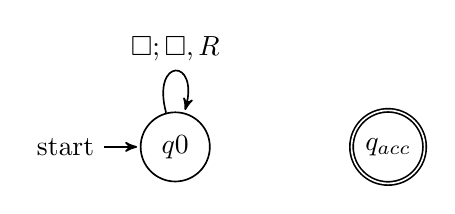
\begin{tikzpicture}[->,>=stealth',shorten >=1pt, auto, node distance=2cm, semithick]
    \tikzstyle{every state}=[text=black, fill=none]
    
    \node[initial,state] (q0)          {$q0$};
    \node[state,accepting]         (qacc) [right of=q0, xshift=20pt] {$q_{acc}$};
    
    \path (q0) edge  [loop above] node {$\square; \square, R$} (qacc)
    ;
  \end{tikzpicture}
\phantom{\hspace{0.8in}}&\hspace{0.8in} 
  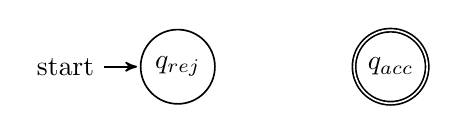
\begin{tikzpicture}[->,>=stealth',shorten >=1pt, auto, node distance=2cm, semithick]
    \tikzstyle{every state}=[text=black, fill=none]
    
    \node[initial,state] (qrej)          {$q_{rej}$};
    \node[state,accepting]         (qacc) [right of=qrej, xshift=20pt] {$q_{acc}$};
  \end{tikzpicture}
  \phantom{\hspace{0.8in}}\\
  Decider? Yes~~~/ ~~~No
  &Decider? Yes~~~/ ~~~No\\
  & \\
  \hline

  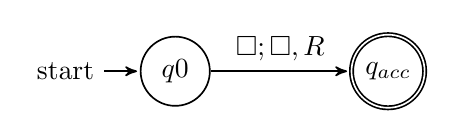
\begin{tikzpicture}[->,>=stealth',shorten >=1pt, auto, node distance=2cm, semithick]
    \tikzstyle{every state}=[text=black, fill=none]
    
    \node[initial,state] (q0)          {$q0$};
    \node[state,accepting]         (qacc) [right of=q0, xshift=20pt] {$q_{acc}$};

    \path (q0) edge [bend left=0] node {$\square; \square, R$} (qacc)
    ;
  \end{tikzpicture} & 
  
  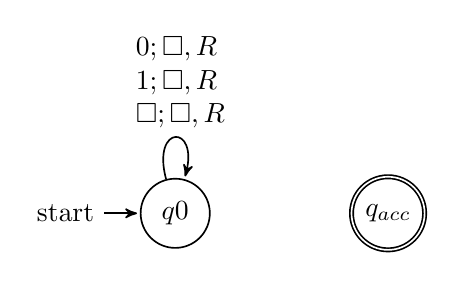
\begin{tikzpicture}[->,>=stealth',shorten >=1pt, auto, node distance=2cm, semithick]
    \tikzstyle{every state}=[text=black, fill=none]
    
    \node[initial,state] (q0)          {$q0$};
    \node[state,accepting]         (qacc) [right of=q0, xshift=20pt] {$q_{acc}$};
    
    \path (q0) edge  [loop above] node {\parbox{1cm}{$0; \square, R$\newline$1; \square, R$\newline $\square; \square, R$}} (q0)
    ;
  \end{tikzpicture}\\
  Decider? Yes~~~/ ~~~No
  &Decider? Yes~~~/ ~~~No\\
  & \\
  
  \hline
  \end{tabular}
  \end{center}
  \newpage

 \vfill
\section*{Day17}




A {\bf Turing-recognizable} language is a set of strings that 
is the language recognized by some Turing machine. We also 
say that such languages are recognizable.

A {\bf Turing-decidable} language is a set of strings that 
is the language recognized by some decider. We also 
say that such languages are decidable.


An {\bf unrecognizable} language is a language that is not Turing-recognizable.

An {\bf undecidable} language is a language that is not Turing-decidable.

\vfill

{\bf  True} or {\bf False}: Any  decidable language  is  also  recognizable.

\vfill

{\bf  True} or {\bf False}: Any  recognizable language  is  also  decidable.

\vfill

{\bf  True} or {\bf False}: Any  undecidable language  is  also  unrecognizable.

\vfill

{\bf  True} or {\bf False}: Any  unrecognizable language  is  also  undecidable.

\vfill

\newpage


{\bf True} or {\bf False}: The class of Turing-decidable languages is closed under complementation.

\vfill

Using formal definition:
\vfill

Using high-level description:
\vfill


{\bf  Church-Turing Thesis} (Sipser p. 183): The informal notion of algorithm is formalized completely  and correctly by the 
formal definition of a  Turing machine. In other words: all reasonably expressive models of 
computation are equally expressive with the standard Turing machine.
 \vfill
\section*{Day18}



Definition: A language $L$ over an  alphabet $\Sigma$ is called {\bf co-recognizable} if its complement,  defined
as $\Sigma^* \setminus L  = \{ x  \in  \Sigma^* \mid x \notin  L \}$, is Turing-recognizable.

{\it Notation}: The complement  of a set $X$ is denoted with  a superscript $c$, $X^c$, or an overline,  $\overline{X}$.

{\bf  Theorem} (Sipser Theorem 4.22): A  language is Turing-decidable if and only if both  it and its complement
are Turing-recognizable.

{\bf Proof, first direction:}  Suppose  language  $L$ is  Turing-decidable.   WTS  that both it and its complement 
are Turing-recognizable.

\vfill

{\bf Proof, second direction:}  Suppose  language  $L$ is  Turing-recognizable, and  so is  its complement.   WTS  that $L$
is Turing-decidable.
\vfill




\newpage

\vfill

\vfill

{\bf Dovetailing}: interleaving progress on multiple computations by 
limiting the number of steps each computation makes in each round.
\newpage

{\bf Claim}: If two languages  (over a fixed alphabet  $\Sigma$) are Turing-decidable, then  their union  is  as well.

{\bf Proof}:


\vfill
\newpage

{\bf Claim}: If two languages  (over a fixed alphabet  $\Sigma$) are Turing-recognizable, then  their union  is  as well.

{\bf Proof}:

 \vfill
\section*{Day19}


{\bf The Church-Turing thesis posits that each algorithm can be implemented by some Turing machine.}

{\bf Describing  algorithms} (Sipser p. 185) To define a Turing machine, we could give a 
\begin{itemize}
\item {\bf Formal definition}: the $7$-tuple of parameters including set of states, 
input alphabet, tape alphabet, transition function, start state, accept state, and reject state.
This is the low-level programming view that models the logic computation flow in a processor.
\item {\bf Implementation-level definition}: English prose that describes the Turing machine head 
movements relative to contents of tape, and conditions for accepting / rejecting based on those contents.
This level describes memory management and implementing data access with data structures.
  \begin{itemize}
    \item Mention the tape or its contents (e.g.\ ``Scan the tape from left to right until a blank is seen.'')
    \item Mention the tape head (e.g.\ ``Return the tape head to the left end of the tape.'')
  \end{itemize}
\item {\bf High-level description} of algorithm executed by Turing machine: 
description of algorithm (precise sequence of instructions), 
without implementation details of machine. 
High-level descriptions of  Turing machine algorithms are written as indented text within quotation marks.   
Stages of the algorithm are typically numbered consecutively.
The first line specifies the input to the machine, which must be a string.
  \begin{itemize}
    \item Use other Turing machines as subroutines (e.g.\ ``Run $M$ on $w$'')
    \item Build new machines from existing machines using previously shown results (e.g.\ 
    ``Given NFA $A$ construct an NFA $B$ such that $L(B) = \overline{L(A)}$'')
    \item Use previously shown conversions and constructions (e.g.\ ``Convert regular expression $R$ 
    to an NFA $N$'')
  \end{itemize}
\end{itemize}

{\bf Formatted inputs to Turing machine algorithms}

The input to a Turing machine is always a string. 
The format of the input to a Turing machine can be checked to interpret 
this string as representing structured data (like a csv file, the formal definition of a DFA, another Turing machine, etc.)


This string may be the encoding of some object or  list of  objects.  

{\bf Notation:} $\langle O \rangle$ is the string that encodes the object $O$.
$\langle O_1, \ldots, O_n \rangle$ is the string that encodes the list of objects $O_1, \ldots, O_n$.

{\bf Assumption}: There are algorithms (Turing  machines) that can be called as subroutines
to decode the string representations of common objects and  interact with these objects as intended
(data structures). These algorithms are able to ``type-check'' and string representations for different
data structures are unique.
  
\newpage
For example, since there are algorithms to answer each of the following questions,
by Church-Turing thesis, there is a Turing machine that accepts exactly those strings for which the 
answer to the question is ``yes''
\begin{itemize}
    \item Does a string over $\{0,1\}$ have even length?

    \item Does a string over $\{0,1\}$ encode a string of ASCII characters?\footnote{An introduction to ASCII 
    is available on the w3 tutorial \href{https://www.w3schools.com/charsets/ref_html_ascii.asp}{here}.}

    \item Does a DFA have a specific number of states?

    \item Do two NFAs have any state names in common?

    \item Do two CFGs have the same start variable?

  \end{itemize}



A {\bf computational problem} is decidable iff language encoding its positive problem instances
is decidable.

The computational problem ``Does a specific DFA accept a given string?'' is encoded by the language
\begin{align*}
  &\{ \textrm{representations of DFAs $M$ and strings $w$ such that $w \in L(M)$}\}  \\
  =& \{ \langle M, w \rangle \mid M \textrm{ is a DFA}, w \textrm{ is a string}, w \in L(M) \}
\end{align*}

The computational problem ``Is the language generated by a CFG empty?'' is encoded by the language
\begin{align*}
  &\{ \textrm{representations of CFGs $G$  such that $L(G) = \emptyset$}\}  \\
  =& \{ \langle G \rangle \mid G \textrm{ is a CFG},  L(G) = \emptyset \}
\end{align*}



The computational problem ``Is the given Turing machine a decider?'' is encoded by the language
\begin{align*}
  &\{ \textrm{representations of TMs $M$  such that $M$ halts on every input}\}  \\
  =& \{ \langle M \rangle \mid M \textrm{ is a TM and for each string } w, \textrm{$M$ halts on $w$} \}
\end{align*}


{\it Note: writing down the language encoding a computational problem is only the first step in 
determining if it's recognizable, decidable, or \ldots }

Deciding a computational problem means building / defining a Turing 
machine that recognizes the language encoding the computational problem, and that 
is a decider.


Some classes of computational problems will 
help us understand the differences between the machine models we've been studying. (Sipser Section 4.1)

    \begin{center}
    \begin{tabular}{|lcl|}
    \hline
    \multicolumn{3}{|l|}{{\bf  Acceptance problem} } \\
    & & \\
    \ldots for DFA & $A_{DFA}$ & $\{ \langle B,w \rangle \mid  \text{$B$ is a  DFA that accepts input 
    string $w$}\}$ \\
    \ldots for NFA & $A_{NFA}$ & $\{ \langle B,w \rangle \mid  \text{$B$ is a  NFA that accepts input 
    string $w$}\}$ \\
    \ldots for regular expressions & $A_{REX}$ & $\{ \langle R,w \rangle \mid  \text{$R$ is a  regular
    expression that generates input string $w$}\}$ \\
    \ldots for CFG & $A_{CFG}$ & $\{ \langle G,w \rangle \mid  \text{$G$ is a context-free grammar 
    that generates input string $w$}\}$ \\
    \ldots for PDA & $A_{PDA}$ & $\{ \langle B,w \rangle \mid  \text{$B$ is a PDA that accepts input string $w$}\}$ \\
    & & \\
    \hline
    \multicolumn{3}{|l|}{{\bf Language emptiness  testing} } \\
    & & \\
    \ldots for DFA & $E_{DFA}$ & $\{ \langle A \rangle \mid  \text{$A$ is a  DFA and  $L(A) = \emptyset$\}}$ \\
    \ldots for NFA & $E_{NFA}$ & $\{ \langle A\rangle \mid  \text{$A$ is a NFA and  $L(A) = \emptyset$\}}$ \\
    \ldots for regular expressions & $E_{REX}$ & $\{ \langle R \rangle \mid  \text{$R$ is a  regular
    expression and  $L(R) = \emptyset$\}}$ \\
    \ldots for CFG & $E_{CFG}$ & $\{ \langle G \rangle \mid  \text{$G$ is a context-free grammar 
    and  $L(G) = \emptyset$\}}$ \\
    \ldots for PDA & $E_{PDA}$ & $\{ \langle A \rangle \mid  \text{$A$ is a PDA and  $L(A) = \emptyset$\}}$ \\
    & & \\
    \hline
    \multicolumn{3}{|l|}{{\bf Language equality testing} } \\
    & & \\
    \ldots for DFA & $EQ_{DFA}$ & $\{ \langle A, B \rangle \mid  \text{$A$ and $B$ are DFAs and  $L(A) =L(B)$\}}$\\
    \ldots for NFA & $EQ_{NFA}$ & $\{ \langle A, B \rangle \mid  \text{$A$ and $B$ are NFAs and  $L(A) =L(B)$\}}$\\
    \ldots for regular expressions & $EQ_{REX}$ & $\{ \langle R, R' \rangle \mid  \text{$R$ and $R'$ are regular
    expressions and  $L(R) =L(R')$\}}$\\
    \ldots for CFG & $EQ_{CFG}$ & $\{ \langle G, G' \rangle \mid  \text{$G$ and $G'$ are CFGs and  $L(G) =L(G')$\}}$ \\
    \ldots for PDA & $EQ_{PDA}$ & $\{ \langle A, B \rangle \mid  \text{$A$ and $B$ are PDAs and  $L(A) =L(B)$\}}$ \\
    \hline
    \end{tabular}
    \end{center}
    

    Example strings in $A_{DFA}$
    
    \vfill
    
    Example strings in  $E_{DFA}$
    
    \vfill
    
    Example strings in  $EQ_{DFA}$
    
    \vfill

    \begin{quote}
      $M_1 = $ ``On input $\langle M,w\rangle$, where $M$ is a DFA and $w$ is a string:
      \begin{enumerate}
      \setcounter{enumi}{-1}
      \item Type check encoding to check input is correct type. If not, reject.
      \item Simulate $M$ on input $w$ (by keeping track of states in $M$, transition function of $M$, etc.) 
      \item If the simulation ends in an accept state of $M$, accept. If it ends in a non-accept state of $M$, reject. "
      \end{enumerate}
      \end{quote}
      
    
    What is $L(M_1)$? 
    
    \vfill
    
    Is $M_1$ a decider?
    
    \vfill
    
    
    {\it Alternate description}:
    Sometimes omit step 0 from listing and do implicit type check.
    
    Synonyms: ``Simulate'', ``run'', ``call''.
    
    \newpage
    
      True / False: $A_{REX} = A_{NFA} = A_{DFA}$
    
      True / False: $A_{REX} \cap A_{NFA} = \emptyset$, $A_{REX} \cap A_{DFA} = \emptyset$, $A_{DFA} \cap A_{NFA} = \emptyset$
    
      
      \vfill
    
      $E_{DFA} = \{ \langle A \rangle \mid  \text{$A$ is a  DFA and  $L(A) = \emptyset$}\}$. 
        A Turing machine that  decides $E_{DFA}$ is
    
      \begin{multicols}{2}
      \begin{quote}
      $M_2 =  $``On  input  $\langle M\rangle$ where $M$ is a  DFA,
      \begin{enumerate}
      \item For integer  $i = 1, 2, \ldots$
      \item \qquad Let  $s_i$ be the  $i$th string over  the alphabet of  $M$ (ordered in  string order).
      \item \qquad Run $M$ on  input  $s_i$.
      \item \qquad If $M$  accepts,  reject.  If $M$  rejects, increment $i$ and keep going."
      \end{enumerate}
      \end{quote}
      
      \vfill

      \columnbreak
    
    
      \begin{quote}
      $M_3 =  $ `` On  input $\langle M \rangle$ where $M$ is  a  DFA,
      \begin{enumerate}
      \item Mark the start  state  of $M$.
      \item Repeat until no  new states get marked:
      \item \qquad Loop over the states of $M$. 
      \item \qquad Mark any unmarked  state  that  has an incoming  edge  from a marked state.
      \item If  no  accept state of $M$ is  marked, $\underline{\phantom{FILL  IN}}$;  otherwise, 
      $\underline{\phantom{FILL  IN}}$".
      \end{enumerate}
      \end{quote}
    \end{multicols}
      
    \vfill
    
    \newpage

    To build a Turing machine that decides $EQ_{DFA}$, notice that 
    \[
    L_1 = L_2 \qquad\textrm{iff}\qquad (~(L_1 \cap \overline{L_2}) \cup (L_2 \cap \overline L_1)~) = \emptyset  
    \]
    {\it There are no elements that are in one set and not the other}
    
    
    $M_{EQDFA} = $ 
    
    
      \vfill
      
    
      {\bf Summary}:  We can use the decision procedures (Turing machines) of decidable problems
      as subroutines in other algorithms. For example, we have subroutines for deciding each of 
      $A_{DFA}$, $E_{DFA}$, $EQ_{DFA}$.  We can also use algorithms for known constructions
      as subroutines in other algorithms. For example, we have subroutines for: counting the number 
      of states in a state diagram, counting the number of characters in an alphabet, converting DFA
      to a DFA recognizing the complement of the original language or a DFA recognizing the 
      Kleene star of the original language, constructing a DFA or NFA from two DFA or NFA so that 
      we have a machine recognizing the language of the union (or intersection, concatenation)
      of the languages of the original machines; converting regular expressions to equivalent DFA; 
      converting DFA to equivalent regular expressions, etc.
     \vfill
\end{document}